\documentclass[11pt]{report}
\usepackage{graphics}
\usepackage{anysize}
\marginsize{3cm}{3cm}{3cm}{2cm}
\def\thesection{\arabic{section}} 
\pagenumbering{Roman}
\renewcommand{\contentsname}
{
\centering
ANNE User Guide
\\ \LARGE APPENDIX A of ANNE Report
\\ \LARGE Table of Contents
}

\begin{document}
\tableofcontents
\newpage
\section{User Guide}
\subsection{Screen Layout}
{
\begin{figure}[t]
\centering
\scalebox{0.4} {
	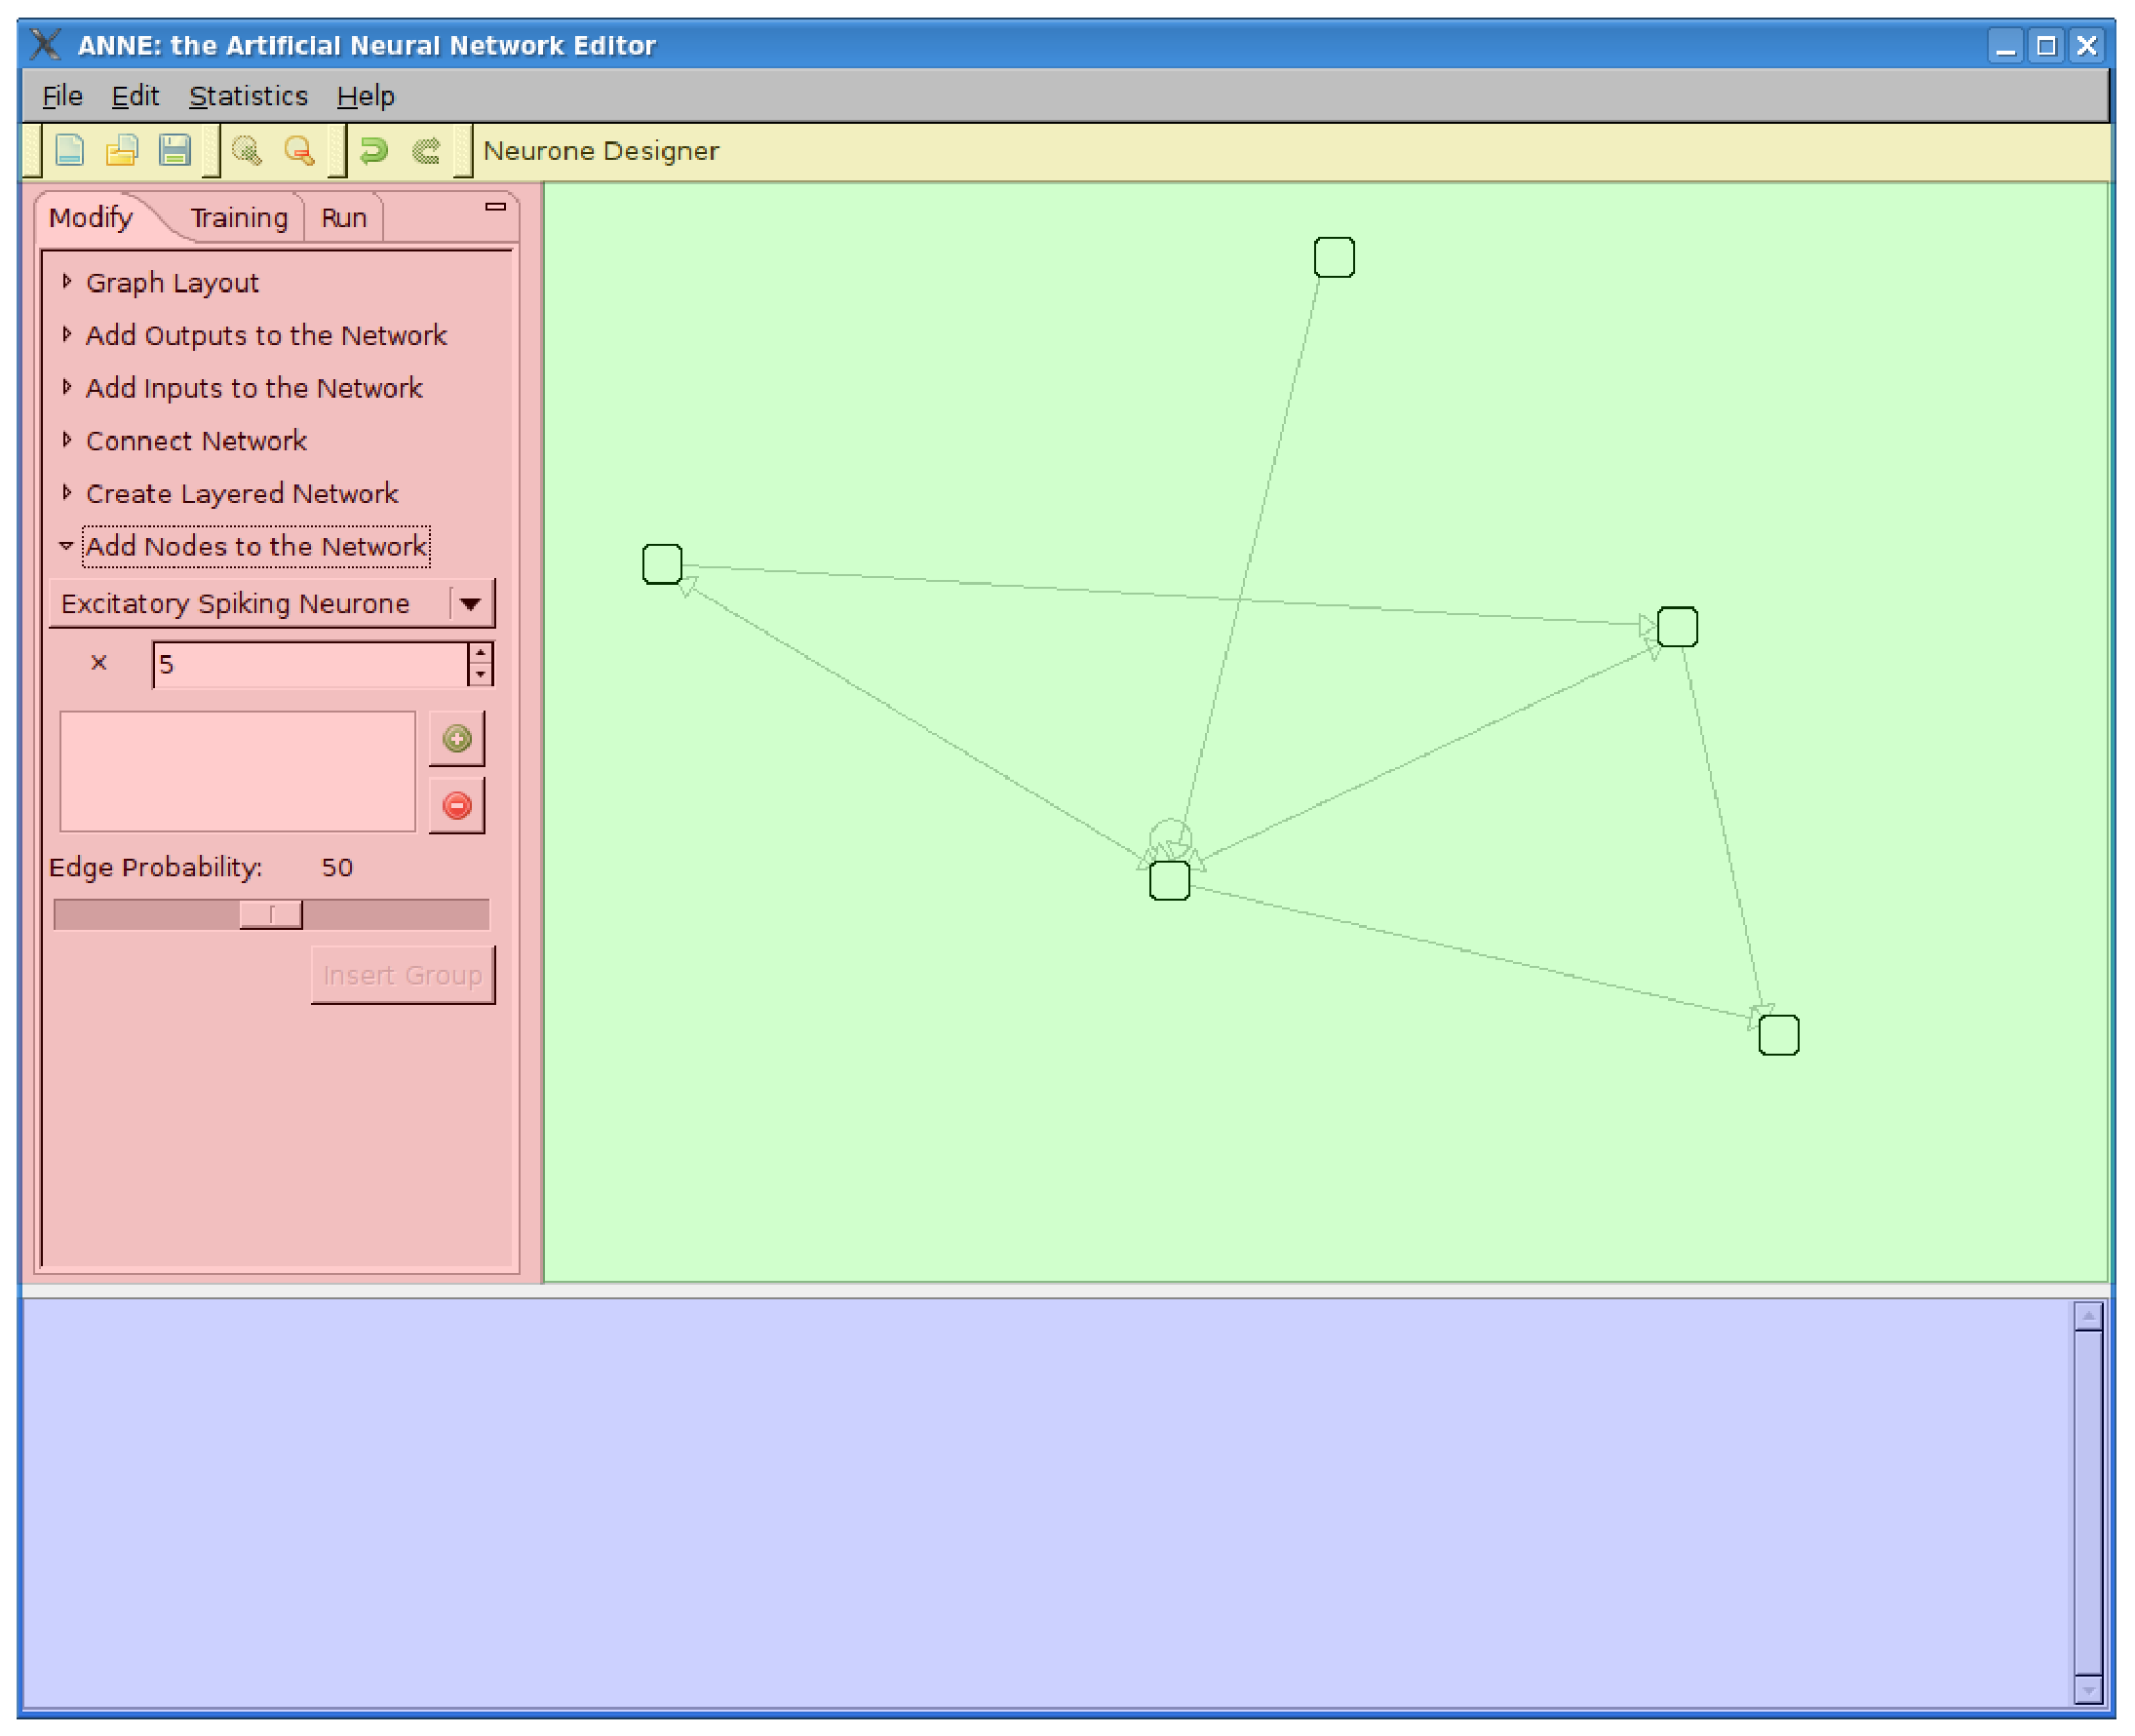
\includegraphics{layout}
}
\caption{ANNE Screen Layout}
\label{fig:layout}
\end{figure}
The main window of ANNE is divided into several panels: the {\textbf{main panel}}, the {\textbf{sidebar}}, the {\textbf{top panel}} and the {\textbf{logging panel}}.

\noindent
In the middle of the screen is the main panel, which is highlighted in green on the diagram. it shows the current view of the network you are editing.

\noindent
The sidebar is on the left of the screen, and is shown in red on the diagram. It contains three tabs: {\textbf{Modify}}, which lets you create and modify your network; {\textbf{Training}}, which allows you to tran your network using a variety of techniques; and {\textbf{Run}}, which lets you run your network.

\noindent
The top panel contains the menu and the toolbar. The menu, shown in grey on the diagram, lets you perform features such as saving and loading files, and enabling and disabling statisticians. The most common menu tasks, such as zooming in and undoing changes, are shown as buttons in the toolbar, shown in yellow.

\noindent
The panel at the bottom of the screen is the logging panel, which is highlighted in blue on the diagram. This displays helpful logging messages after certain tasks have been executed.
}
\newpage
\subsection{Creating a Group of Neurones}
{
\begin{figure}[t]
\centering
\scalebox{0.4} {
	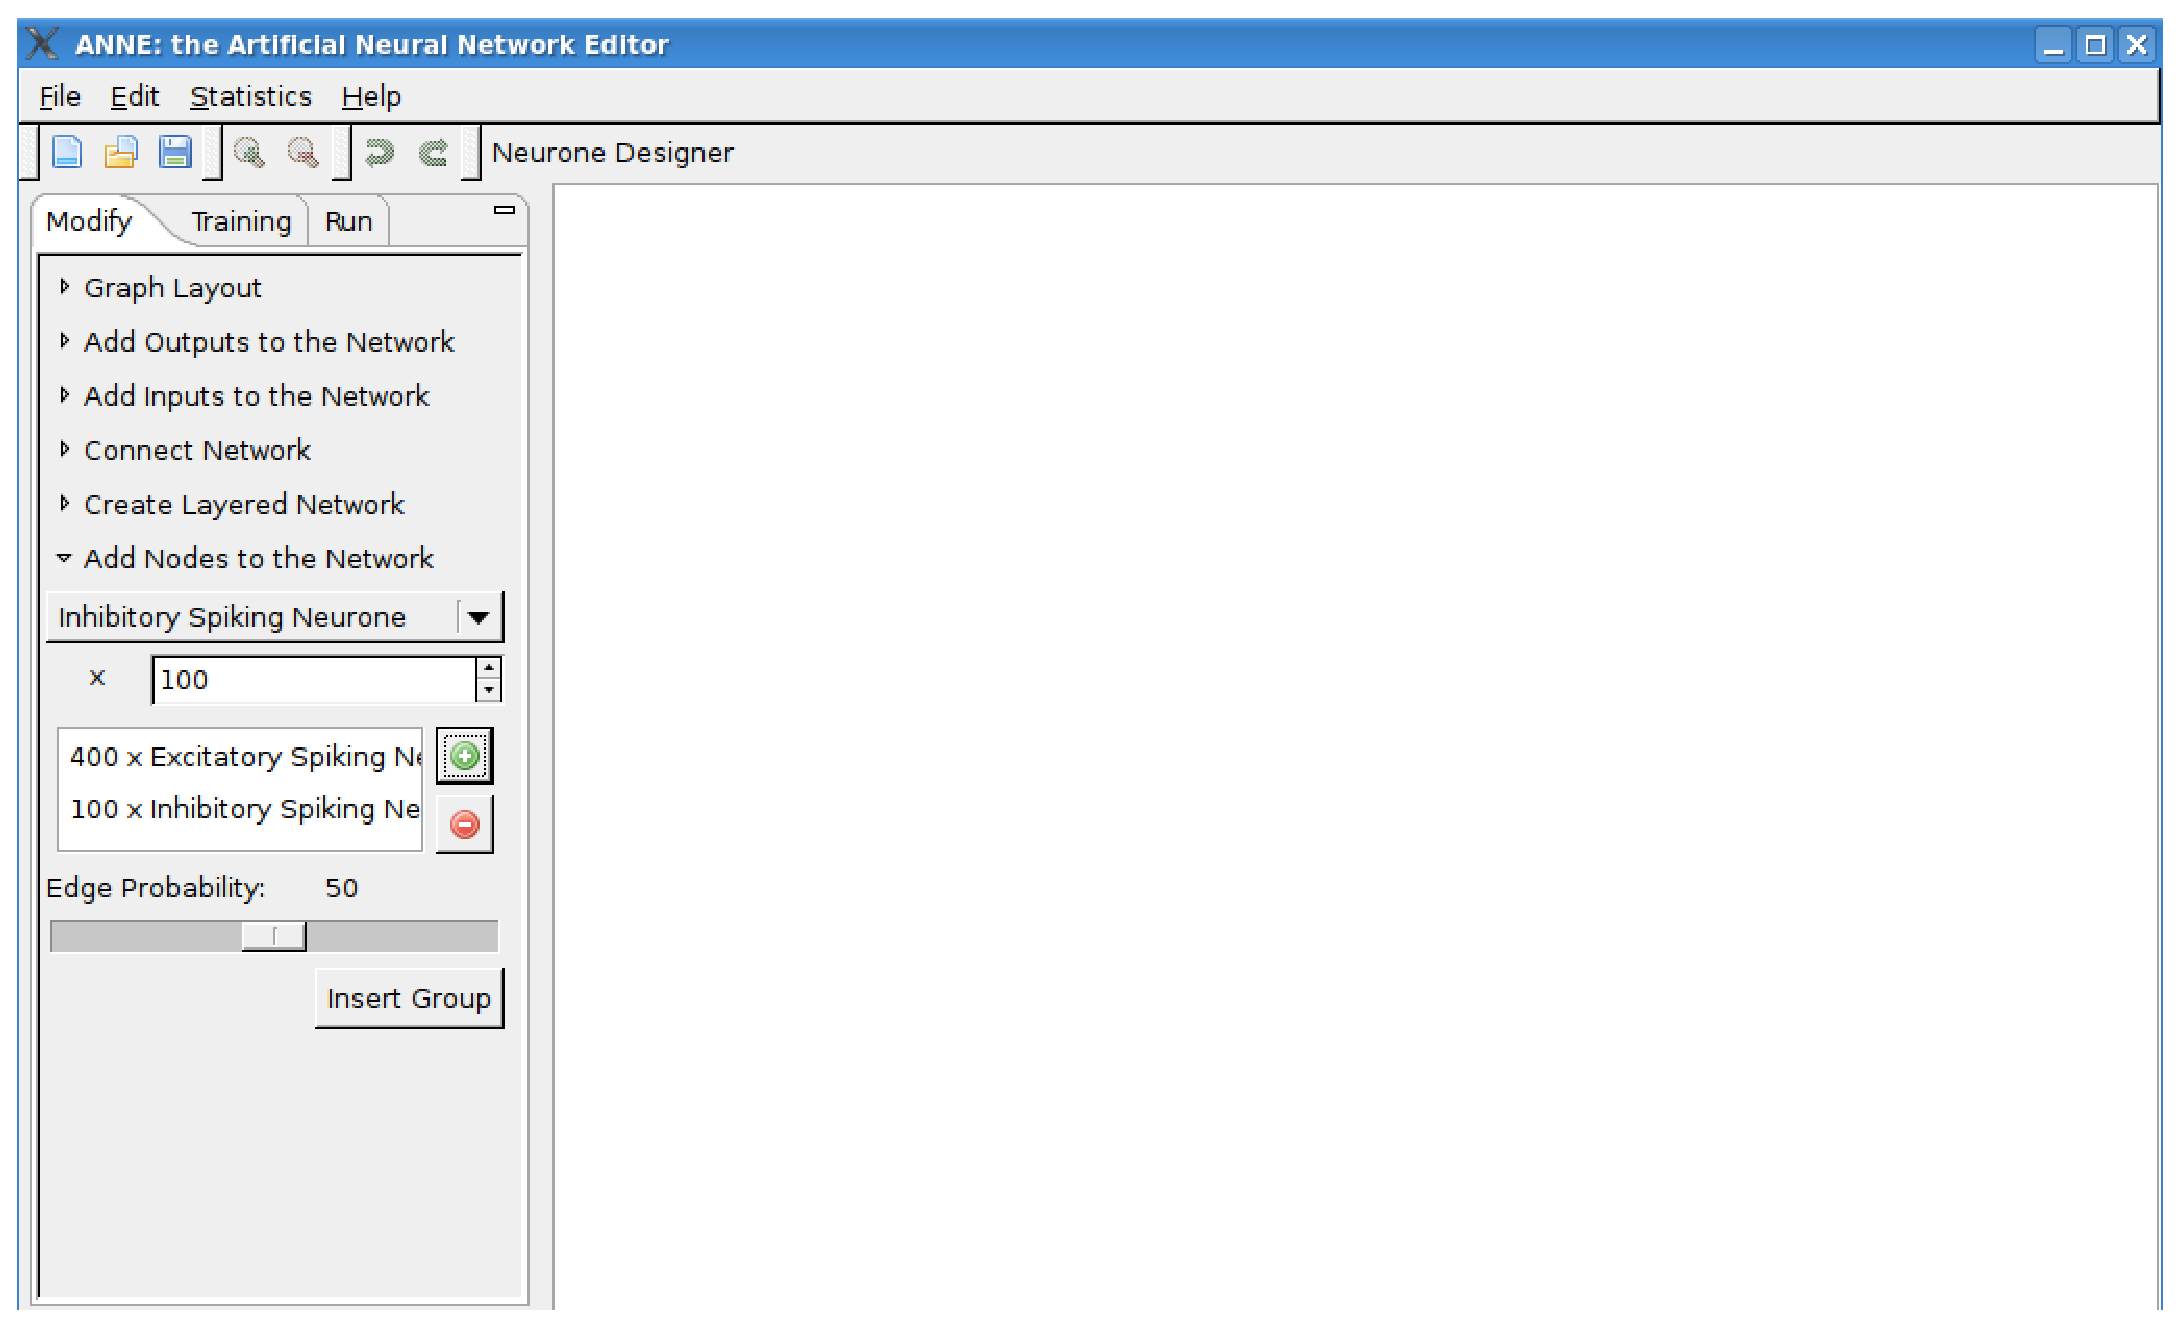
\includegraphics{addNodes}
}
\caption{The Add Nodes Panel}
\label{fig:addnodes}
\end{figure}
When ANNE is first opened, it contains an empty neural network. Therefore, the first thing to do is add some neurones. To do this, go to the Modify Panel in the sidebar and then select the ``Add Nodes to the Network" option. Choose the type of neural network you would like to add. Next, choose the number of neurones you would like in the neural network. To add this group to the graph, select the ``add group" button (the green plus sign) and then click ``Insert Group" to add them to the graph. To see the resulting neurones, you can zoom into this neural network by clicking the neural network and then pressing the ``Zoom In" button in the toolbar.
}
\newpage
\subsection{Creating Input Neurones}
{
To create input nodes, select the ``Add Inputs to Network" option in the Modify Tab. Next, select the type of input node you would like to use. If ``PunchInput" is selected, a dialog box will appear prompting you to select the number of input nodes you would like to insert. If ``DATInput" is selected, you will be prompted to with an open dialog box to select a {\textit{.dat}} file to use.

\begin{figure}[t]
\centering
\scalebox{0.4} {
	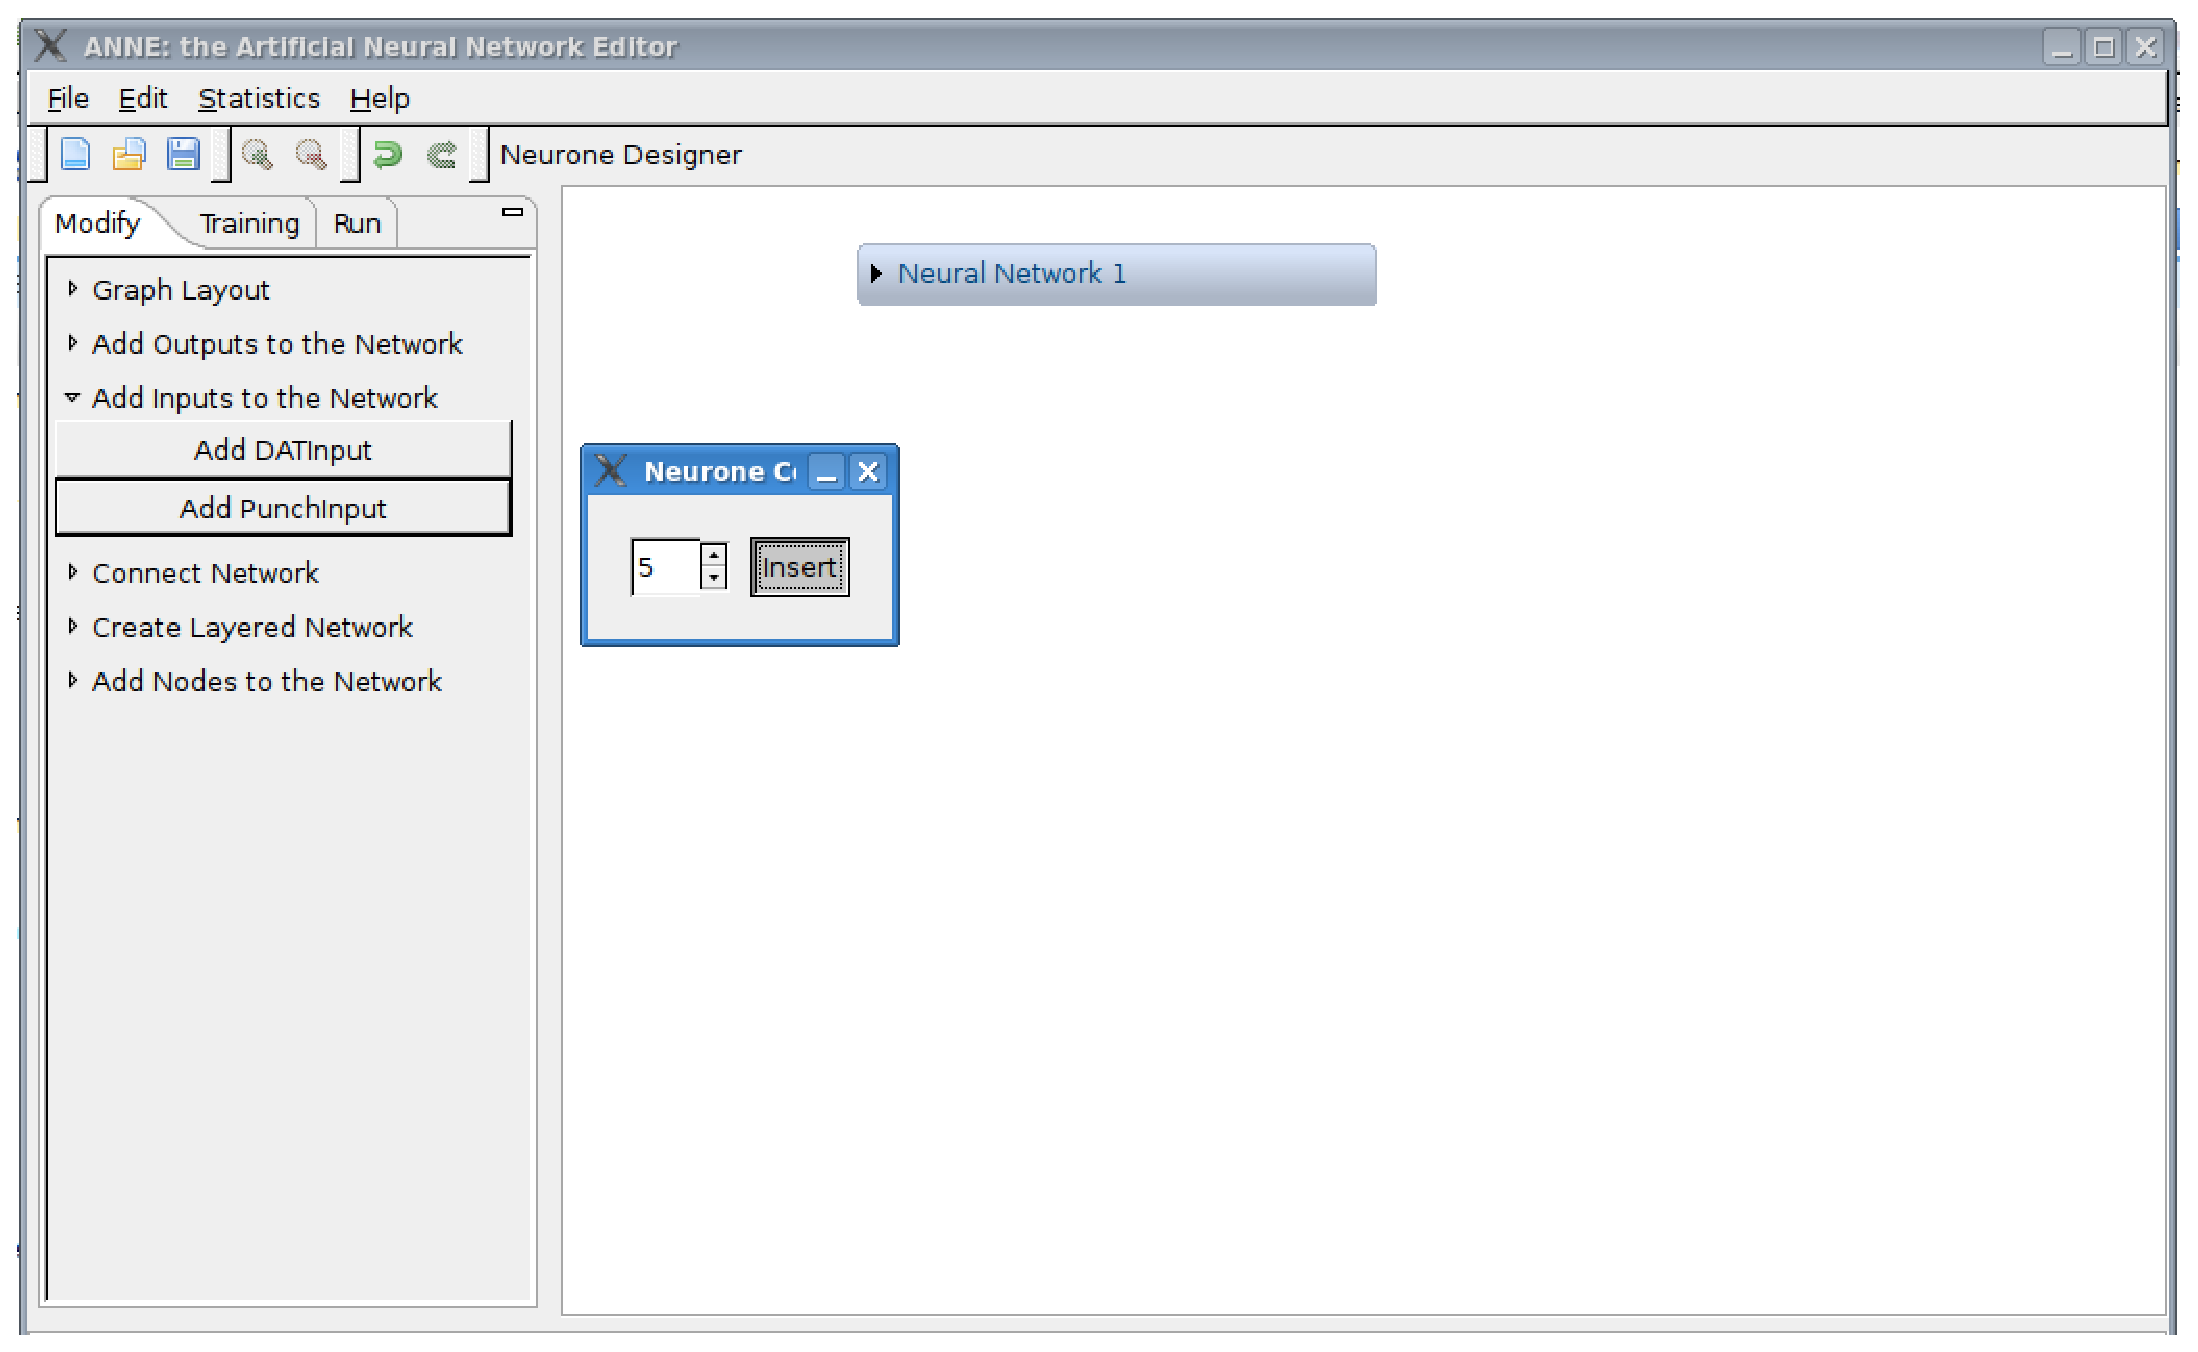
\includegraphics{addInput}
}
\caption{The Add Inputs to Network Panel}
\label{fig:addinputs}
\end{figure}
}
\newpage
\subsection{Connecting Networks}
{
To connect a group of neurones or neural networks, you will need to use the ``Connect Network" panel in the Modify tab. To select which nodes you wish to connect, click the add button and then select the nodes you would like to connect together by dragging a box around them with the mouse, or by clicking on them directly. You can select the probablity of the edges being generated by using the slider, and the algorithm to use from the drop{}-down menu. Once you are happy with your selection and options, click the ``Go" button to generate the edges that connect the nodes together.

\begin{figure}[t]
\centering
\scalebox{0.4} {
	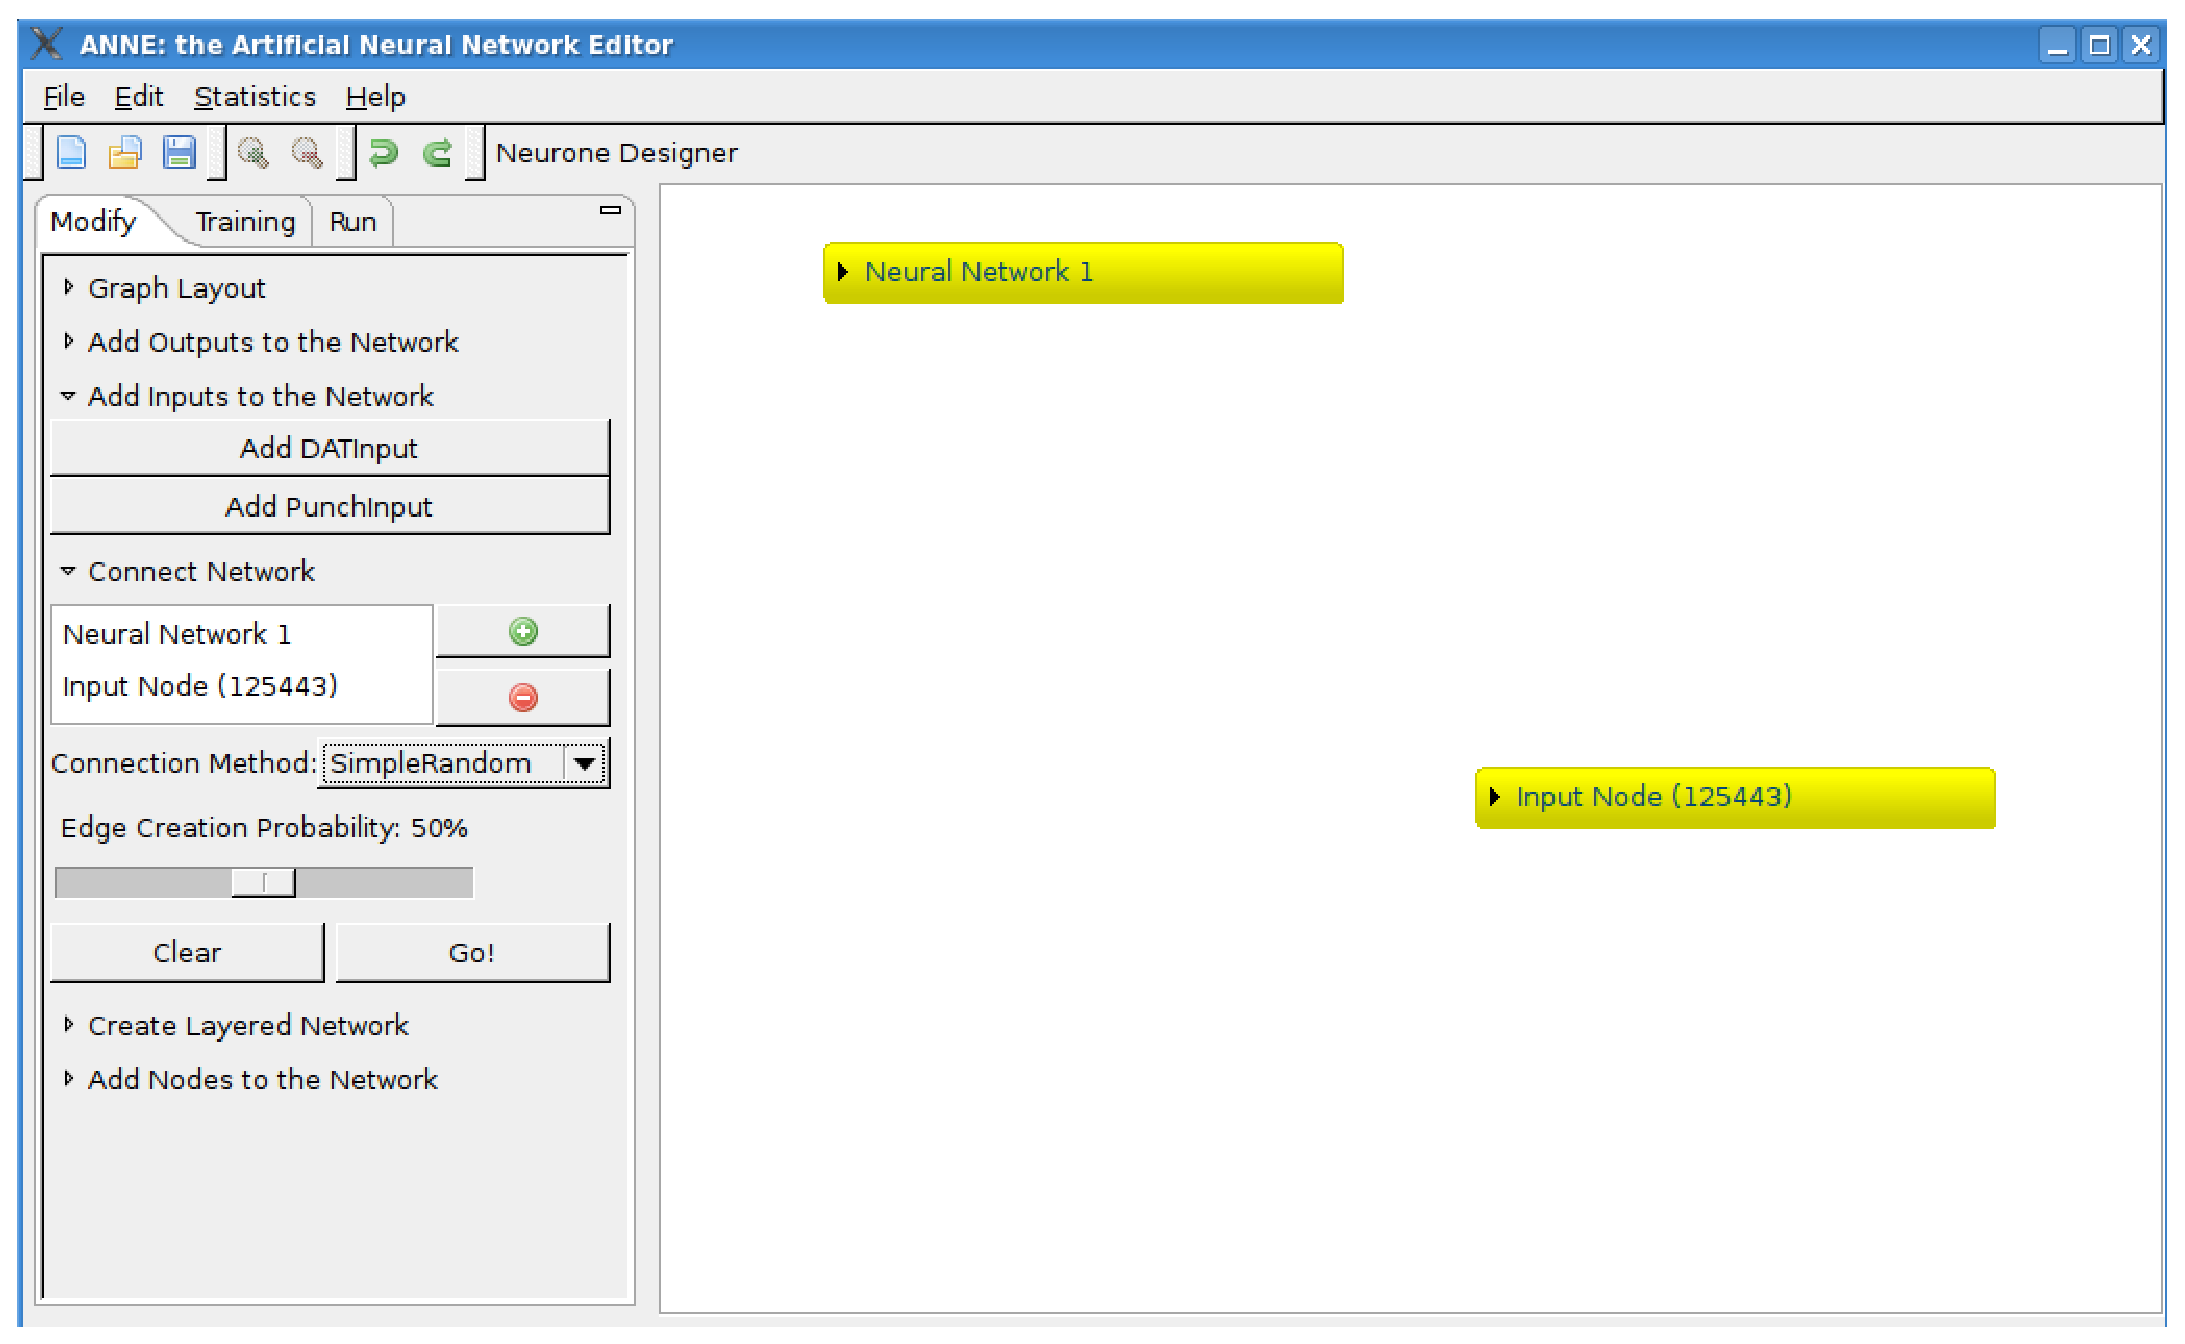
\includegraphics{connect}
}
\caption{Connecting Networks}
\label{fig:connect}
\end{figure}
}
\newpage
\subsection{Training and Simulating a Network}
{
Once you have finished editing your network, it can be trained and simulated. The example network we are using consists of two PunchingInput neurones, two groups of quiet excitatory spiking neurones, and a group containing a mixture of quiet excitatory and quiet inhibitory spiking neurones.

\begin{figure}[t]
\centering
\scalebox{0.4} {
	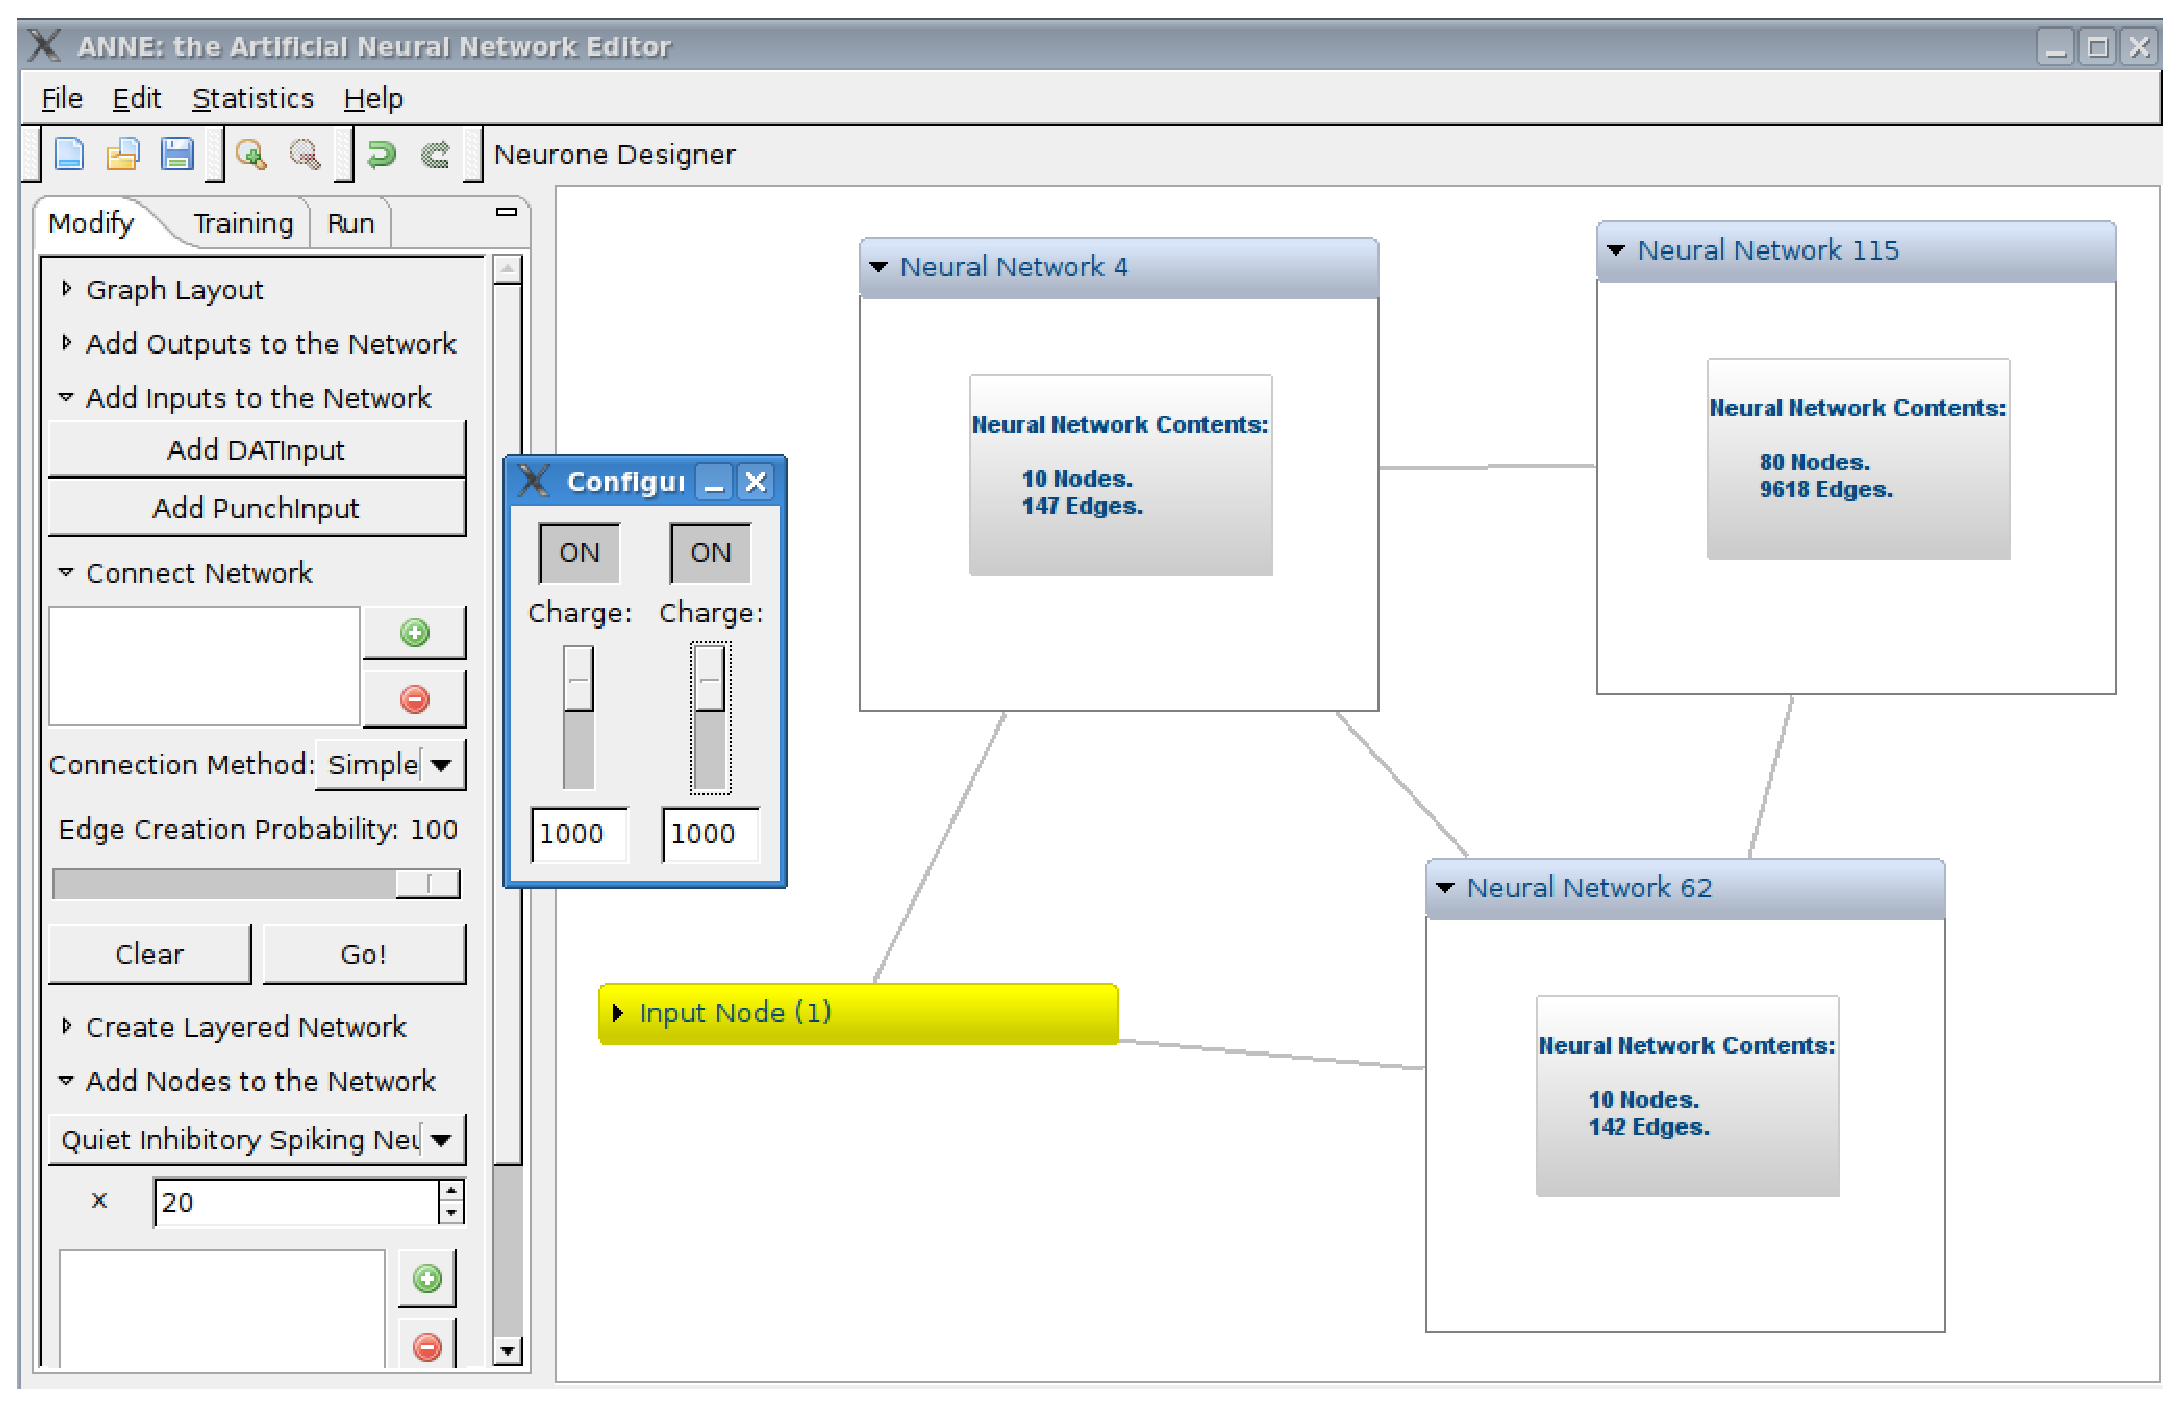
\includegraphics{example}
}
\caption{Example Network}
\label{fig:eg}
\end{figure}
}
\newpage
\subsection{Training}
{
Now that the network has been created, a real{}-time plot of its activity can be made by selecting ``Statistics" then enabling ``RealTimePlot" from the menu. When you train and run your network, its activity will be shown in the plot window that is created. This can be navigated using your arrow keys; $\uparrow$ and $\downarrow$ zoom in and out respectively, and $\leftarrow$ and $\rightarrow$ will pan the plot left and right.

\noindent
To train the network, first open the Train tab in the sidebar. Click the ``Select Input Node" button and click an input node, then change any training parameters as required. The drop-down box in this tab contains the different training algorithms available; in our example, we will use STDP. Click the Start Training button, then wait for the network to finish training. The Real{}-Time plot window can show its progress.

\begin{figure}[t]
\centering
\scalebox{0.4} {
	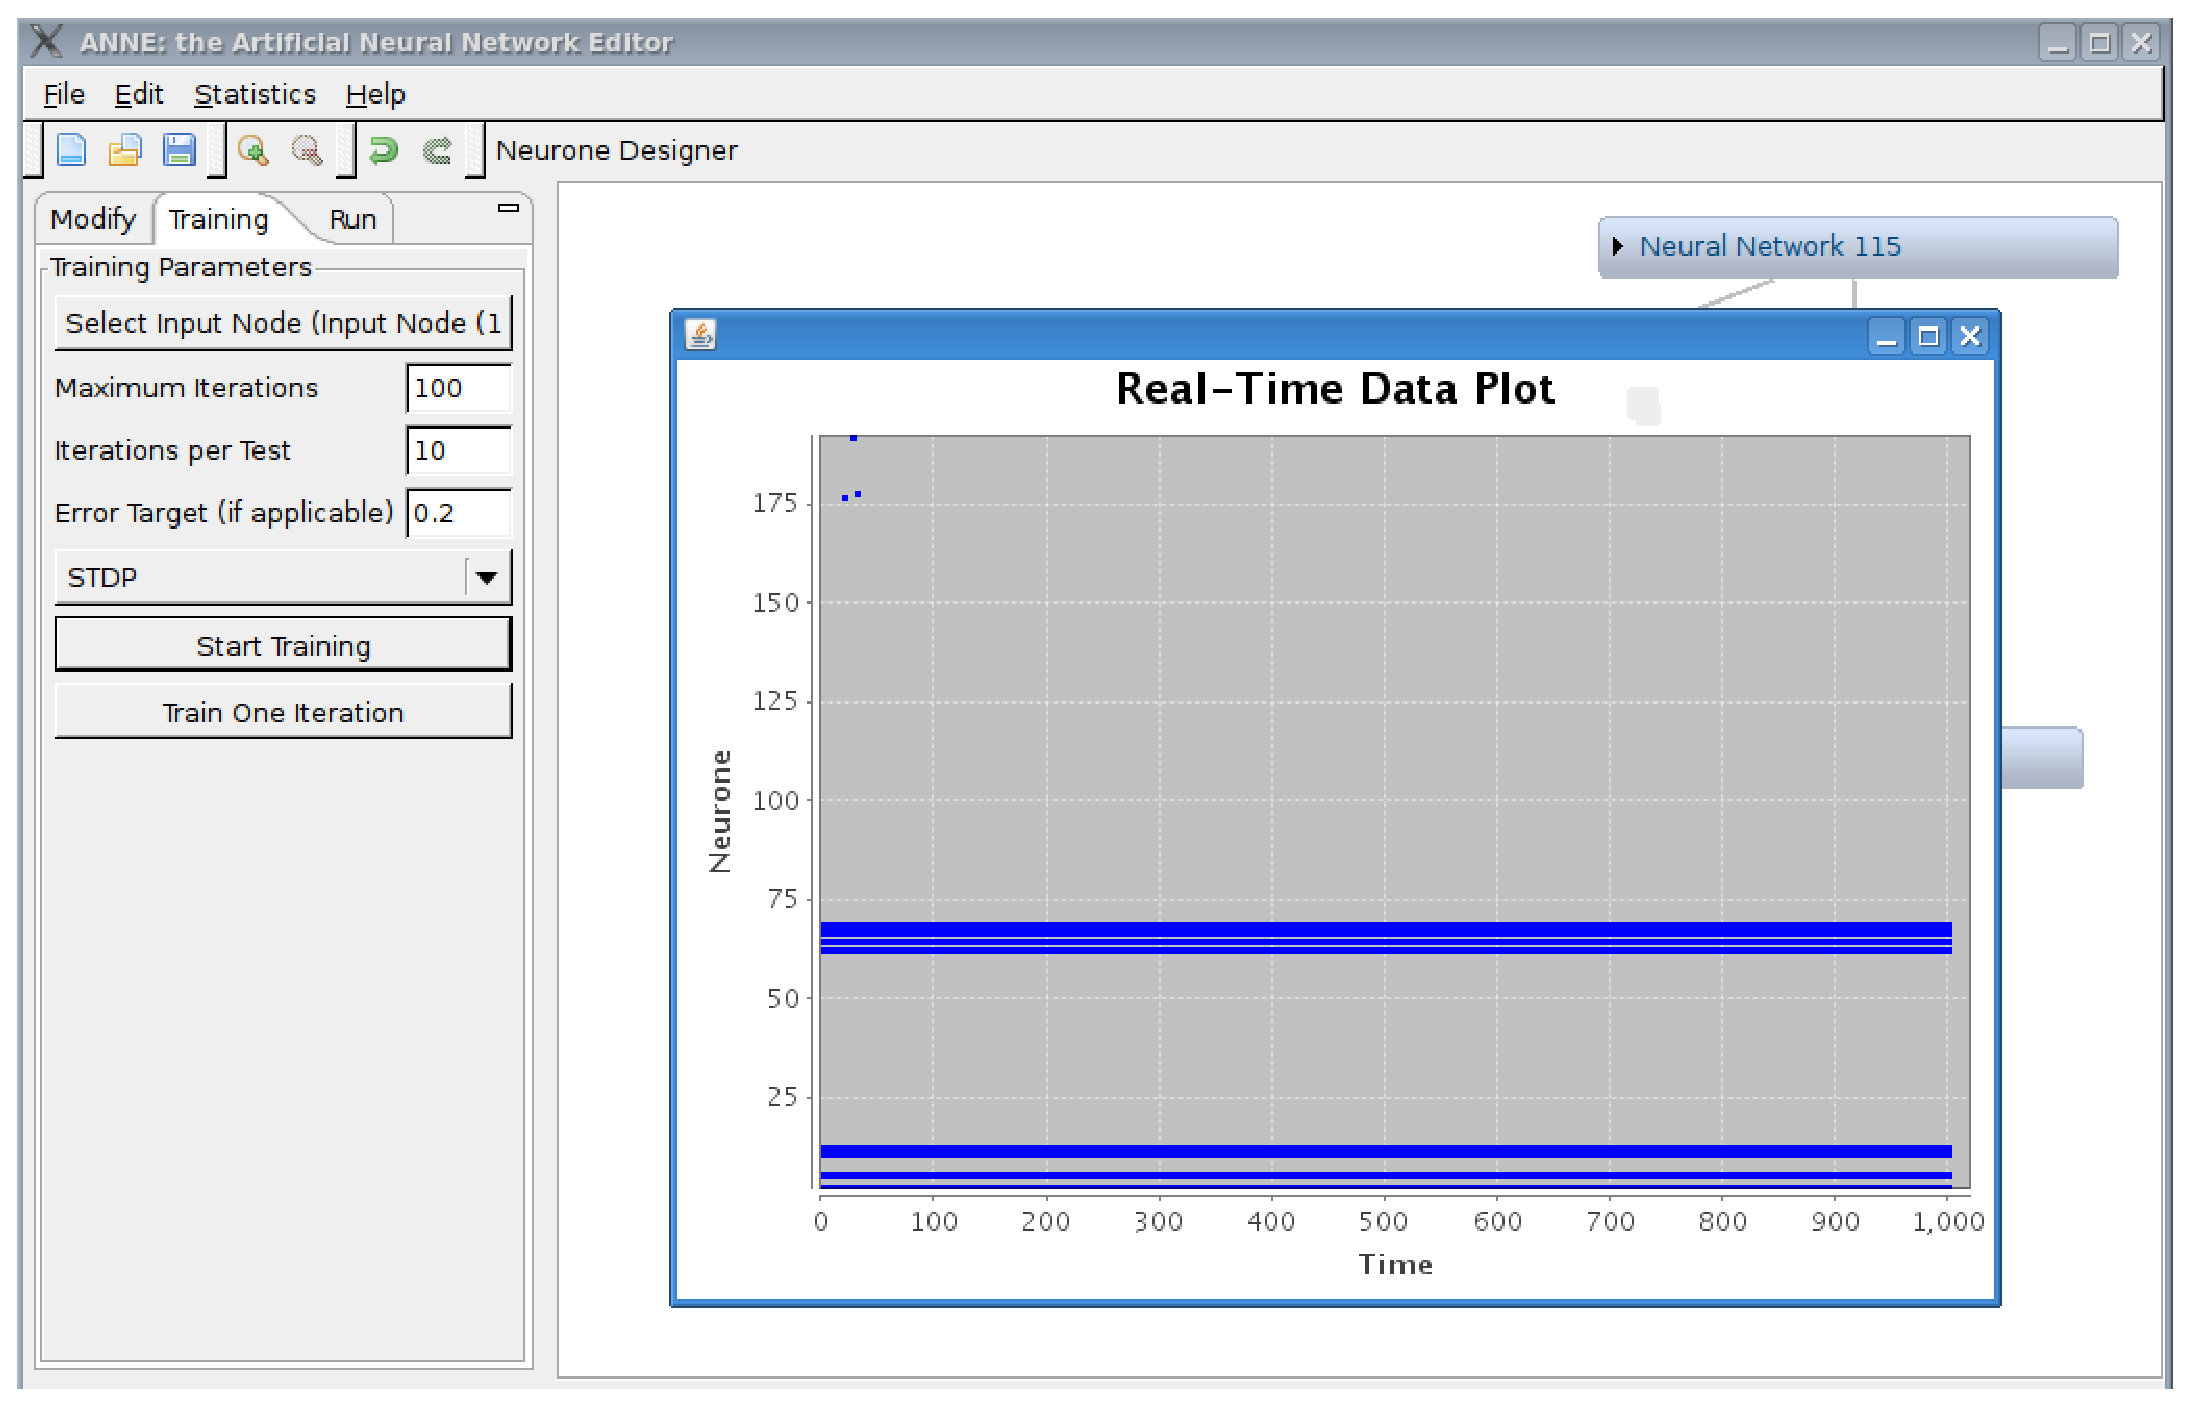
\includegraphics{train}
}
\caption{Training a Network}
\label{fig:train}
\end{figure}
}
\newpage
\subsection{Running Networks}
{
To run your trained network, click on the Run tab in the sidebar. There are options for simulating the network one step at a time, but for now just click the Run button to make the network start running. Now that the simulation has begun, it is possible make changes to the input nodes and observe the results. In our example, clicking the button by one of the input neurones stops it from firing, and the real-time plot shows that the neural network has been sufficiently trained to keep responding as if it were still turned on; it has learned the spatio{}-temporal association between these neurones.

\begin{figure}[t]
\centering
\scalebox{0.35} {
	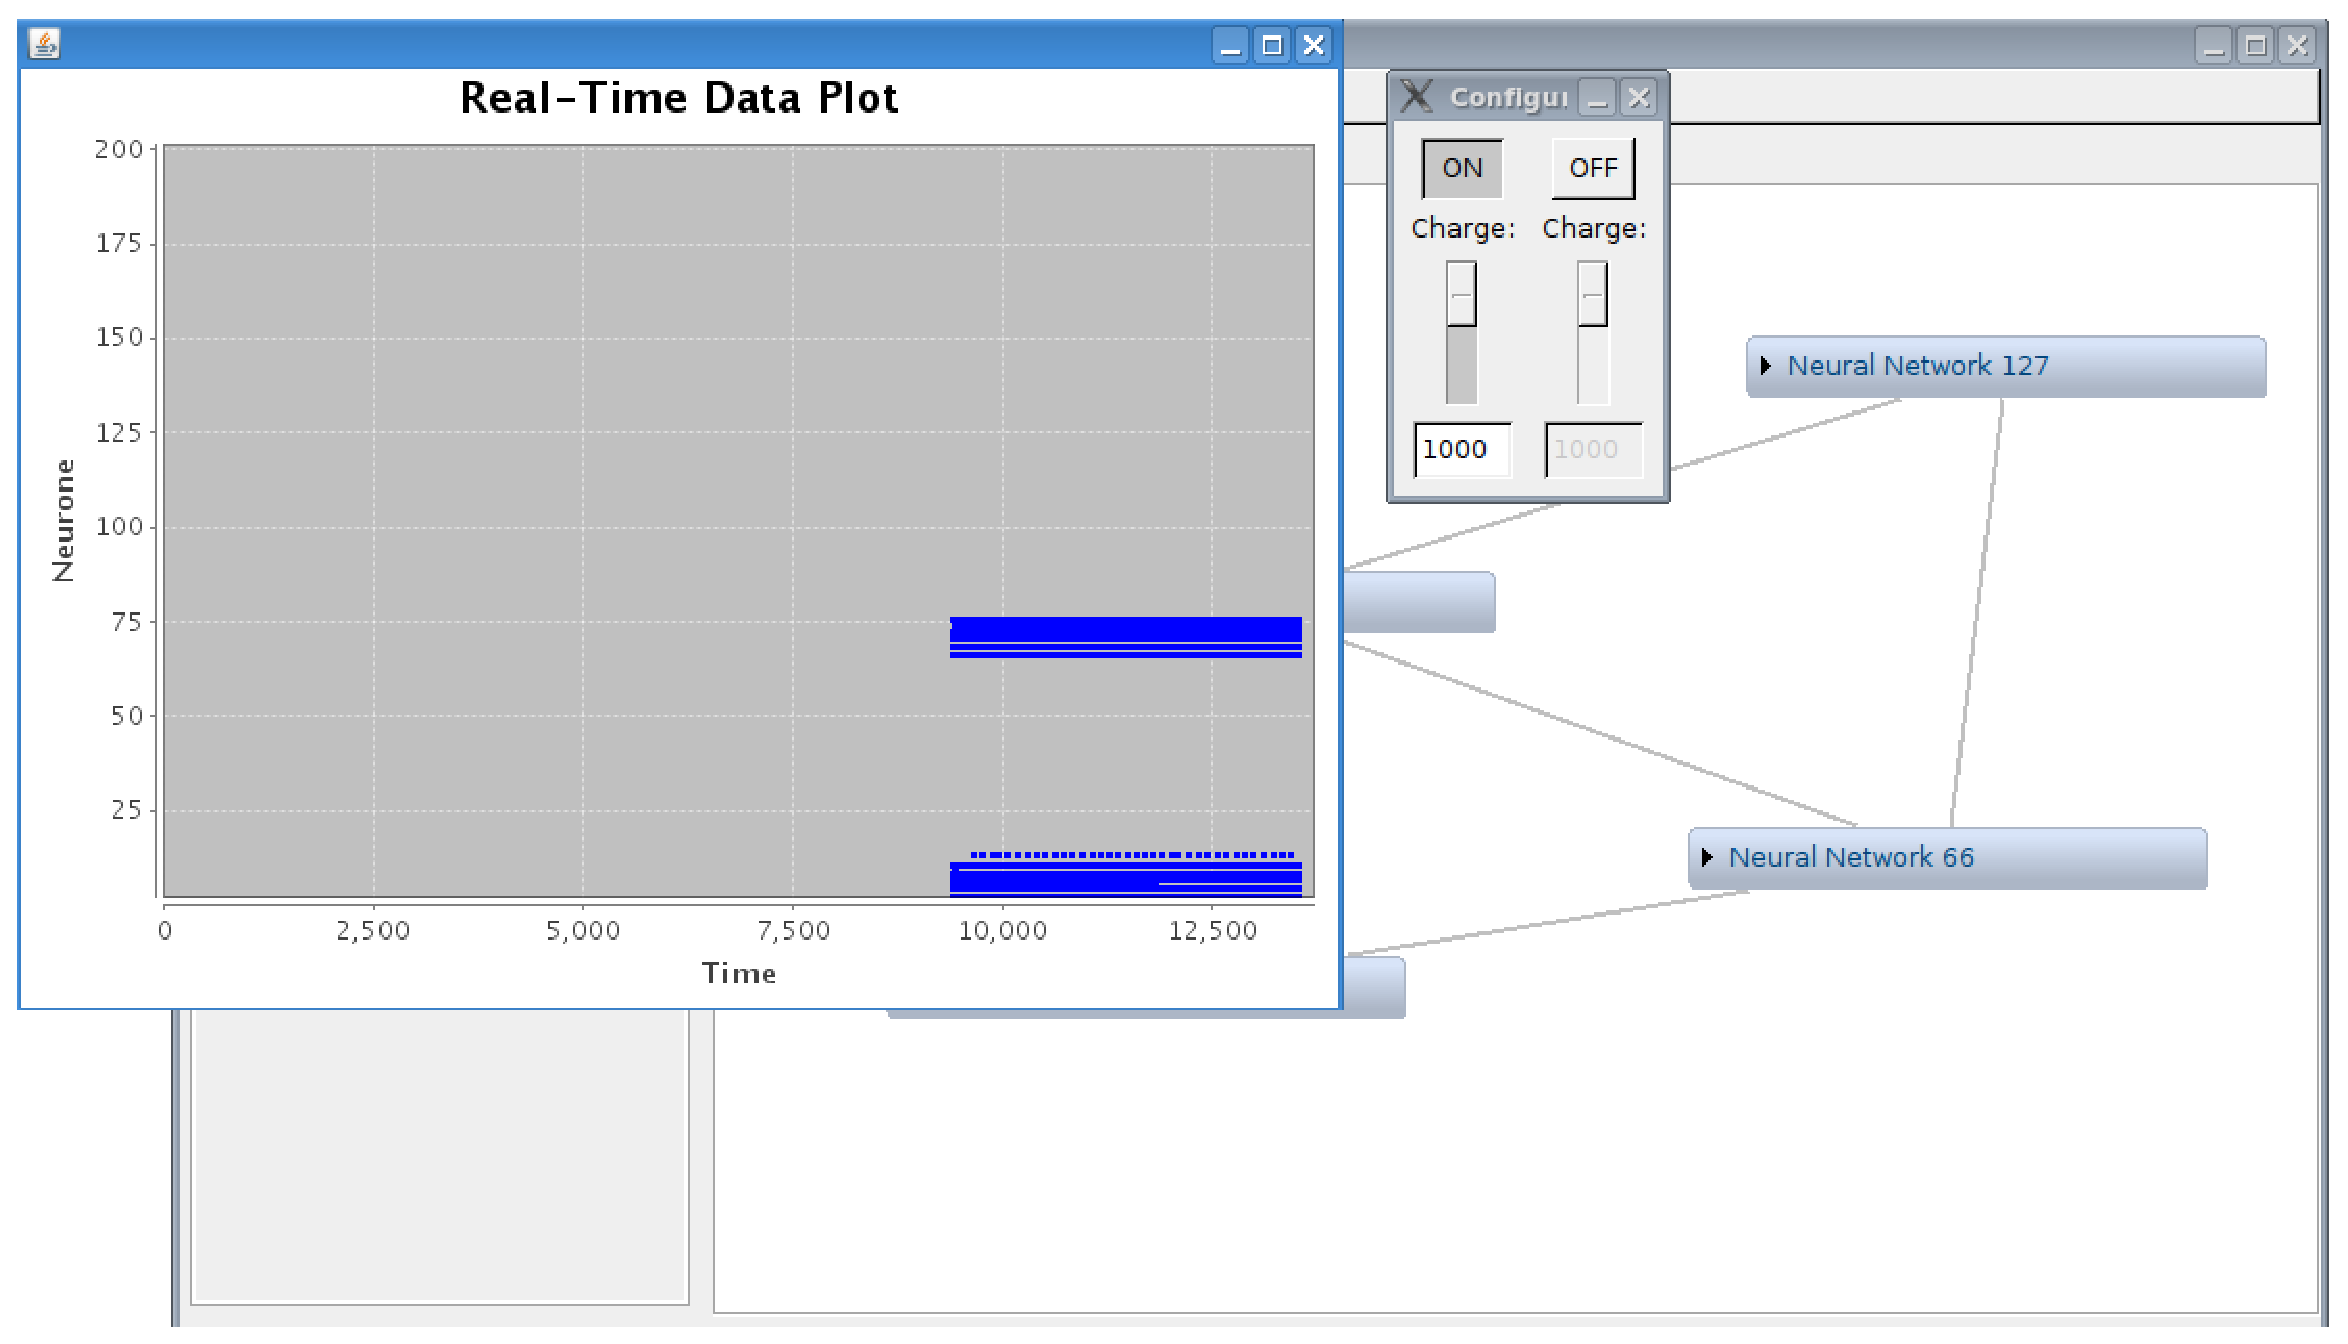
\includegraphics{run}
}
\caption{Running a Network}
\label{fig:run}
\end{figure}
}
\newpage
\subsection{Saving and Loading}
{
Finally, save your changes to the neural network and close the program. Either click ``File" then ``Save as" from the menu, or click the save icon on the toolbar. Once the network has finished saving, close ANNE by either clicking the ``X" icon in the top-right corner of the screen or choosing ``File" then ``Close" from the menu.

\begin{figure}[t]
\centering
\scalebox{0.4} {
	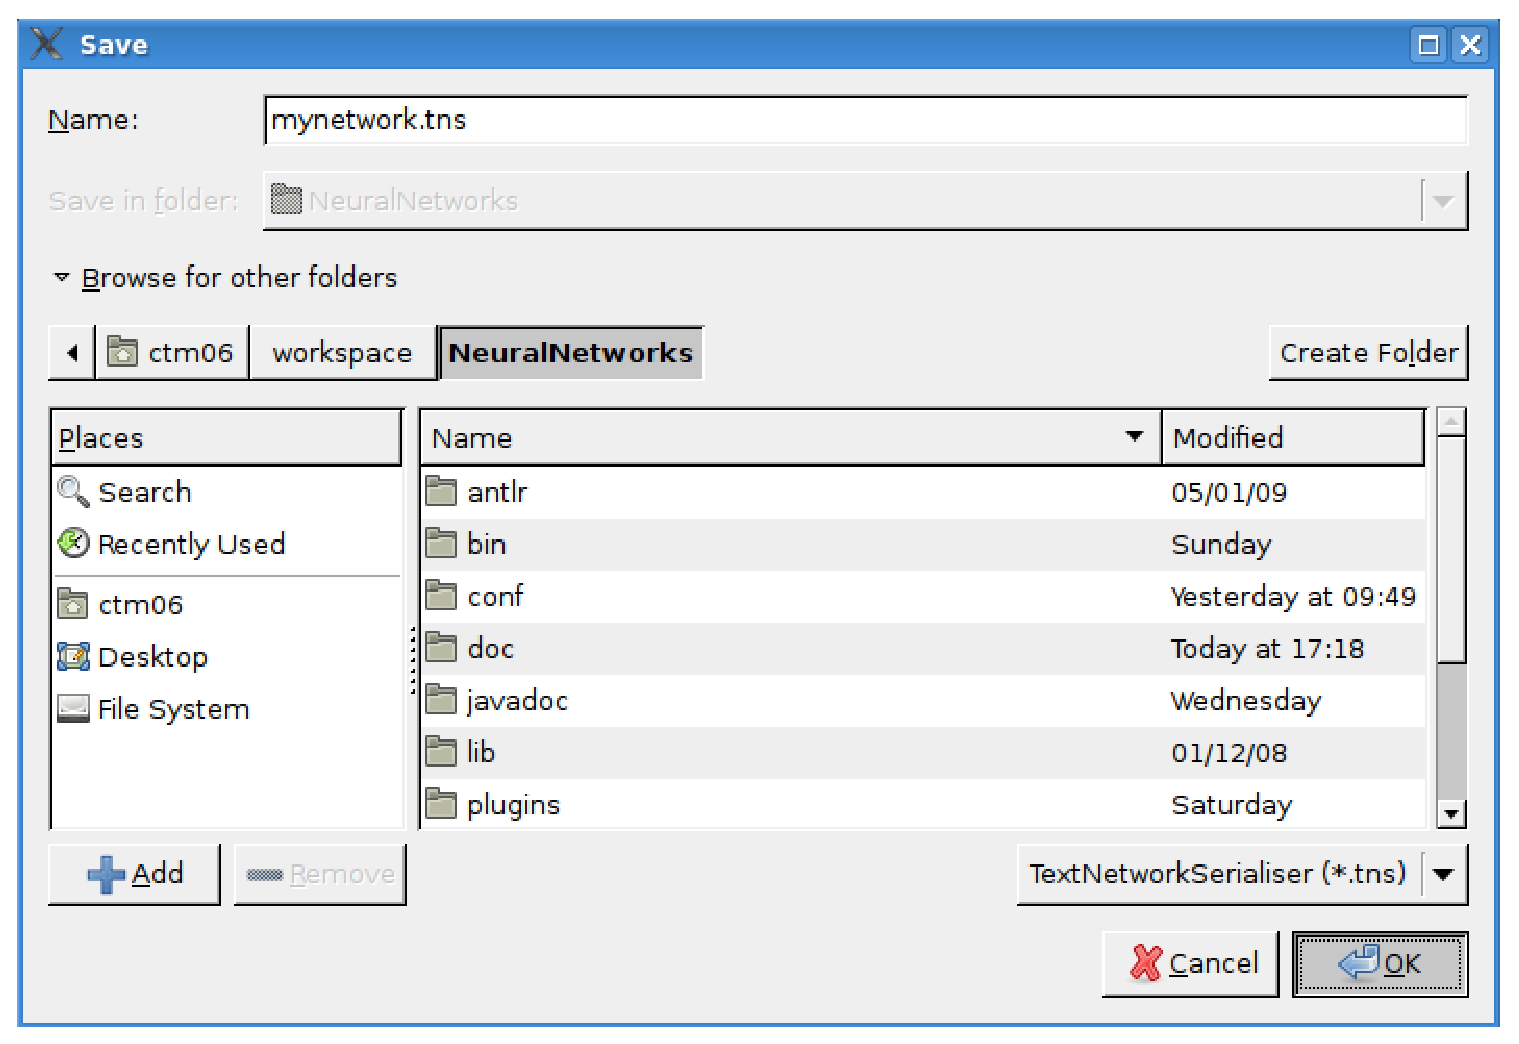
\includegraphics{save}
}
\caption{Saving and Loading Networks}
\label{fig:save}
\end{figure}
}
\end{document}
